\documentclass[MS]{inithesis}
%\documentclass[economy,twoside,bind]{inithesis}
% Use the second for a single-spaced copy suitable for duplex printing
% and binding.

% Other useful options (there are more options documented in Chapter 2):
%  * draft -- don't actually include images, print a black bar on overful
%             hboxes
%  * MS    -- Format for a Master's Thesis.  No UMI abstract page, some 
%             textual changes to title page.  


% Useful packages for thesis writing:
\usepackage{amsmath, amssymb, amsfonts, amsthm}
\usepackage{graphicx}
%\usepackage{natbib}
\usepackage{color}
\usepackage{bm}
%\usepackage{subfigure}
\usepackage{graphicx}
\usepackage{mathabx}
\usepackage{multirow}
\usepackage{setspace}
\usepackage{pdfpages}
\usepackage{tocloft}
\addtolength\cftfignumwidth{2.7em}%
\addtolength\cfttabnumwidth{2.7em}%
%\renewcommand{\cftpartnumwidth}{4em}
%\renewcommand{\cftchapaftersnumb}{\hspace{0em}}
%\renewcommand{\cftsecnumwidth}{1.5em}
%\renewcommand{\cftsecaftersnumb}{\hspace{0em}}
%\renewcommand{\cftsubsubsecindent}{8em}
%\renewcommand{\cftsubsecaftersnumb}{\hspace{0em}}

% \usepackage{cite}  % If you include this, hyperlink cites will
                     % break.  It's nice to use this package if your bibstyle
							% sorts entries by order-of-use, rather than
							% alphabetically (as plain does).
							
%Theorem, Lemma, etc. environments
\newtheorem{theorem}{Theorem}%[section]
\newtheorem{lemma}[theorem]{Lemma}
\newtheorem{proposition}[theorem]{Proposition}
\newtheorem{corollary}[theorem]{Corollary}
\newtheorem{result}[theorem]{Result}

% Personal commands and abbreviations.
%Define and personal commands here

%Graphics Path to find your pictures
\graphicspath{{./Pictures/}}


%-----------------------------------------------------------------------------%
% PREAMBLE 
%-----------------------------------------------------------------------------%
\author{Harshad J Shirwadkar}% First Name, Middle Initial, Last Name
\title{The World Wide Web in the Face of Future Internet
    Architectures}
%\supervisor{Dr. Nicolas Christin}
%\advisor{Dr. Nicolas Christin}
\department{Information Networking Institute} 
\program{Information Networking}% MSISTM, MSIN or MIST-X
%\departmenthead{Dr. Dena Haritos Tsamitis}
%\dean{Dr. Pradeep Khosla}
\previousdegreelist{B.E., Computer Engineering, Pune Institute of
  Computer Technology \\ M.S., Information Networking, Carnegie
  Mellon University}% Separate Multiple Entries with ' \\ '
\fulldate{May, 2016} % Month, Year

% Copyright text.  If undefined, default is 'All rights reserved'
% (Example sets the text to a hyperlinked Creative Commons Licence)
\copyrighttext{ All rights reserved except the rights granted by the\\
   \href{http://creativecommons.org/licenses/by-nc/3.0/us/}
        {Creative Commons Attribution-Noncommercial Licence}
}


%-----------------------------------------------------------------------------%
% HYPERREF: plain black hypertext references for ref's and cite's.
%-----------------------------------------------------------------------------%
\usepackage[pdftex, pdfusetitle, plainpages=false, 
				letterpaper, bookmarks, bookmarksnumbered,
				colorlinks, linkcolor=black, citecolor=black,
	         filecolor=black, urlcolor=black]
				{hyperref}

\begin{document}

% Fill in the blanks in cur_ThesisSig.doc with your information and save in 
% PDF format as signature.pdf 
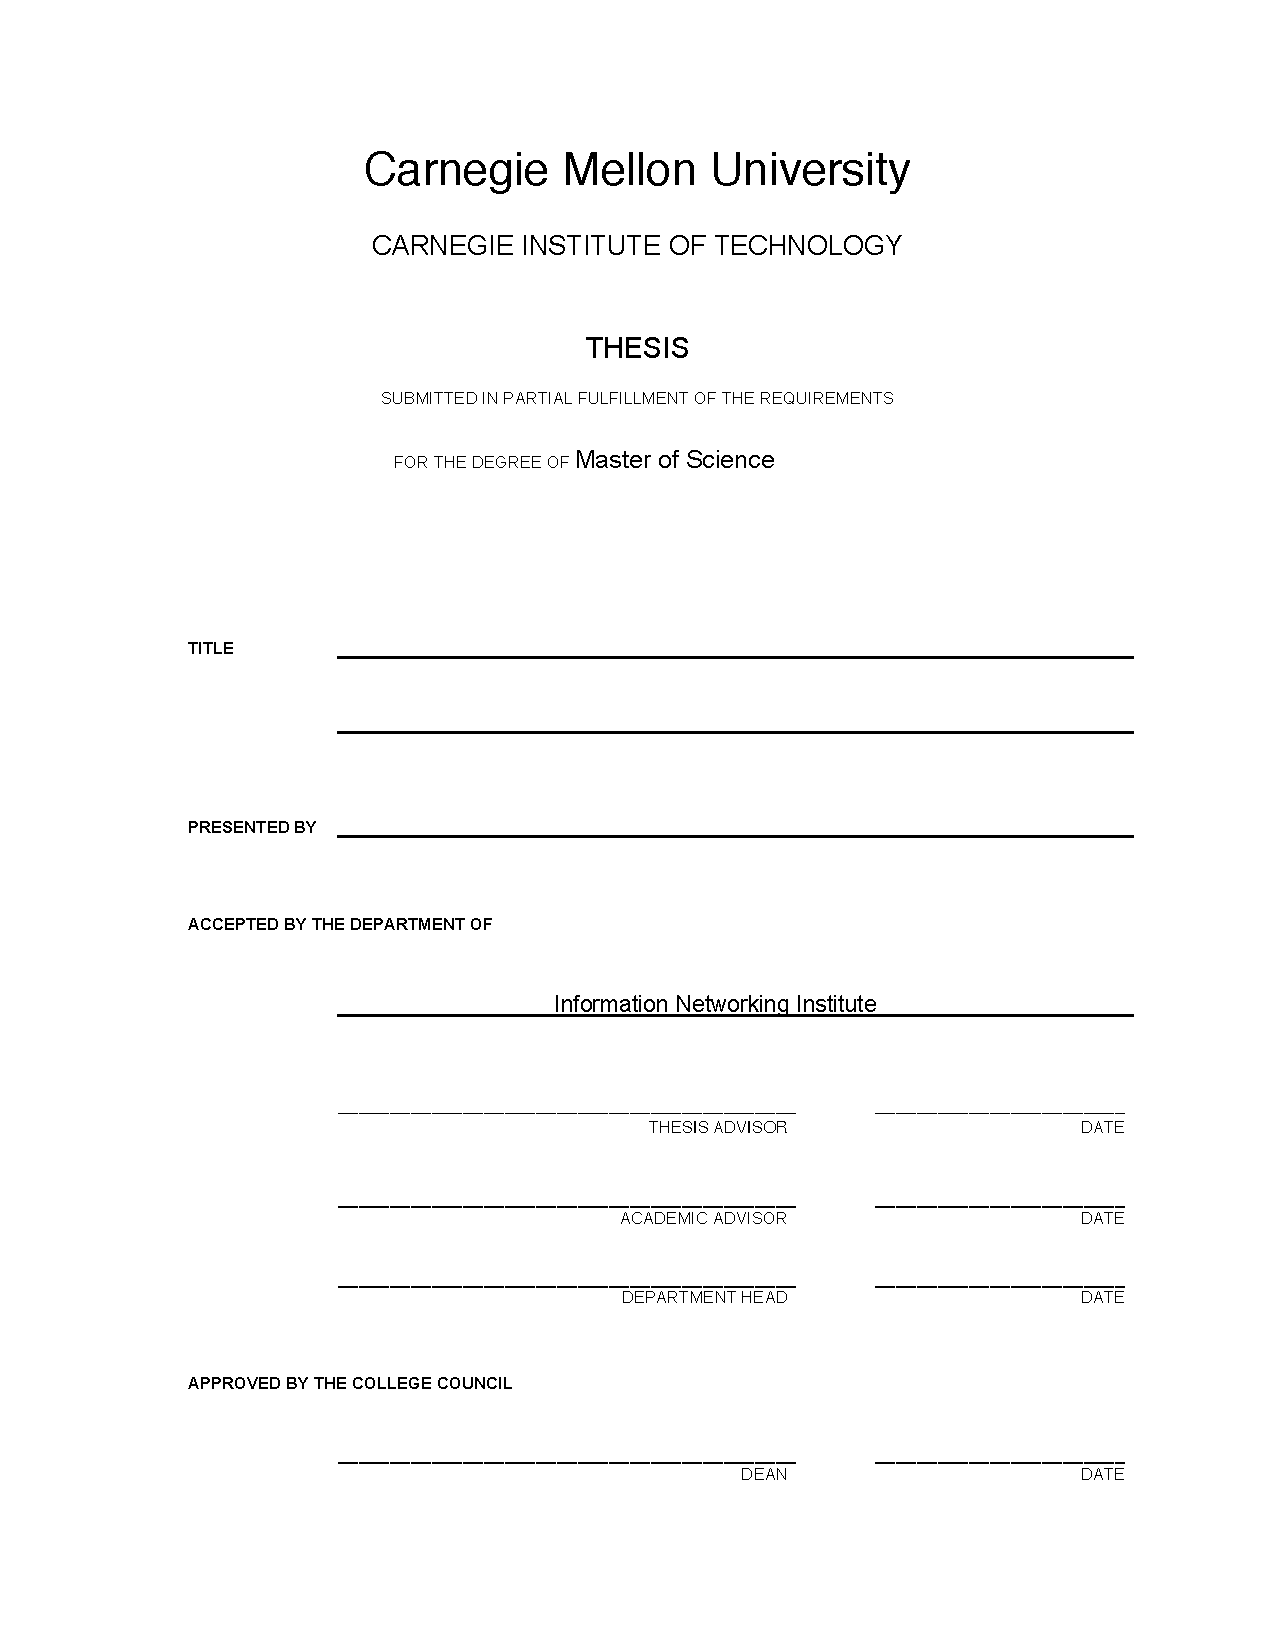
\includepdf[pages={1}]{signature.pdf}

%-----------------------------------------------------------------------------%
% TITLE PAGE -- provides UMI abstract title page & copyright if appropriate
%-----------------------------------------------------------------------------%
\maketitle

%-----------------------------------------------------------------------------%
% ACKNOWLEDGEMENTS -- included file should start with '\acknowledgements'
%-----------------------------------------------------------------------------%
\acknowledgements

\setcounter{page}{2}

Working on master's thesis was my first real research experience. I
thoroughly enjoyed it. It taught me to think about problems in a
different way. I would like to thank everyone who directly or
indirectly supported me throughout this wonderful journey.

I would like to express my deepest gratitude to my advisor, Professor
Peter Steenkiste for his support and guidance throughout the duration
of the project. He was always available to answer my questions and
show me the right way. His continued support over the past two years
has been crucial in this accomplishment. I would also like to
acknowledge Professor Srinivasan Seshsan who served as my thesis
reader and shared valuable feedback on the ideas.

I would like to thank the entire XIA research group for sharing
valuable time to time feedback on my work. I loved being a part of the
group. I would also like to thank Dan Barrett who helped me with
understanding the huge codebase and with setting up various
experiments. His door was always open whenever I ran into a trouble
spot.

Also, I would like to thank Saurabh Kadekodi for many meaningful
discussions that shaped ideas in the thesis.

Finally, I must express my very profound gratitude to my parents and
my brother for providing me with their continuous encouragement and
unfailing support. This work would not have been possible without
them.

This research was funded in part by NSF under awards number
CNS-1040801 and CNS-1345305.

}

%-----------------------------------------------------------------------------%
% ABSTRACT -- included file should start with '\abstract'.
%-----------------------------------------------------------------------------%
\abstract

Write your abstract here.  You should not include references or mathematical notation.}

%-----------------------------------------------------------------------------%
% FRONTMATTER -- ToC is required, LoT and LoF are required if you have any
% tables or figures, respectively. List of Abbreviations and Symbols is 
% optional.
%-----------------------------------------------------------------------------%
\tableofcontents % Automatically generated
\newpage
\listoftables	% If you have any tables, automatically generated
\addcontentsline{toc}{chapter}{List of Tables}%
\newpage
\listoffigures	% If you have any figures, automatically generated
\addcontentsline{toc}{chapter}{List of Figures}%
%\newpage
%\abbreviations

% You can put here what you like, but here's an example
%Note the use of starred section commands here to produce proper division
%headers without bad '0.1' numbers or entries into the Table of Contents.
%Using the {\verb \begin{symbollist} } environment ensures that entries are
%properly spaced.

\section*{Symbols}

Put general notes about symbol usage in text here.  Notice this text is
double-spaced, as required.

\begin{symbollist}
	\item[$\mathbb{X}$] A blackboard bold $X$.  Neat.
	% Optional item argument makes the symbol/abbr
	\item[$\mathcal{X}$] A caligraphic $X$.  Neat.
	\item[$\mathfrak{X}$] A fraktur $X$.  Neat.
	\item[$\mathbf{X}$] A boldface $X$.
	\item[$\mathsf{X}$] A sans-serif $X$. Bad notation.
	\item[$\mathrm{X}$] A roman $X$.
\end{symbollist}

\section*{Abbreviations}

Long lines in the \texttt{symbollist} environment are single spaced, like in
the other front matter tables.

\begin{symbollist}
	\item[AR] Aqua Regia, also known as hydrocloric acid plus a splash of 
	nitric acid.
	\item[SHORT] Notice the change in alignment caused by the label width
	between this list and the one above.  Also notice that this multiline
	description is properly spaced. 
	\item[OMFGTXTMSG4ME] Abbreviations/Symbols in the item are limited to
	about a quarter of the textwidth, so don't pack too much in there.
	You'll bust the margins and it looks really bad.
\end{symbollist}
} % List of Abbreviations. Start file with '\abbreviations'

%==============================================================================
%-----------------------------------------------------------------------------%
%
% MAIN BODY OF PAPER
%
%
%-----------------------------------------------------------------------------%
\chapter{World Wide Web}
\label{chap:www}
The World Wide Web is arguably the most important application of the
Internet. The World Wide Web is an information space that allows
exchanging information objects called web resources between hosts. It
was invented by English scientist Tim Berners-Lee in 1989.

The web is so popular that the term is often used interchangeably with
the Internet itself. However, these two are not the same. The Internet
is a giant network of interconnected computers identified by IP
address. Whereas, the web is a collection of web resources such as
documents, videos, images that these interconnected computers can
network. Essentially, the web runs \emph{on top of} the Internet.

In this chapter we will take a closer look at the important components
of the web.

\section{Universal Resource Identifiers}
The web resources are uniquely identified by something called as
Universal Resource Identifiers or URIs. URI is a string of characters
that can identify a web resource uniquely. This unique identification
provides the network entities a way to identify and therefore
\emph{request} as well as \emph{serve} a resource. RFC 2396 formally
defined the format of URI. The definition was later refined by RFC
3986. The simplified definition of the URI is as follows.
\begin{center}
  \begin{verbatim}
  URI         = scheme : hierarchical-part [ ? query ] [ # fragment ]
  hierarchical-part   = // authority path
                         / path
\end{verbatim}
\end{center}
\begin{itemize}
  \item{\emph{Scheme:}} Examples of popular schemes are HTTP, FTP,
    mailto etc.
  \item{\emph{Hierarchical Part:}} Location of a web resource within
    some logical hierarchy. Often, this part is formed by combining
    the host (a registered name or an IPv4 address) and hierarchical
    path (similar to UNIX file system paths).
  \item{\emph{Query:}} Traditionally consists of key-value pairs.
  \item{\emph{Fragment:}} A character string that identifies a
    fragment in the resource. For example, a section in an article.
\end{itemize}
The example of a URI given in RFC 3986 is as follows.
\begin{verbatim}
foo://example.com:8042/over/there?name=ferret#nose
\_/   \______________/\_________/ \_________/ \__/
 |           |            |            |        |
scheme     authority       path        query   fragment
\end{verbatim}
URL (Universal Resource Locator) is the most commonly used form of URI
in the World Wide Web. In addition to uniquely identifying a web
resource, URL also provides a way to locate the resource. Essentially,
URL identifies a web resource by its network location.
\section{Hypertext Transfer Protocol}
The primary method used for publishing and retrieving these web
resources is Hypertext Transfer Protocol (HTTP). Although HTTP is one
of many Internet communication protocols, the web resources are
usually accessed via HTTP. HTTP is a request-response type of
protocol. The HTTP clients or web clients request resources by sending
a \texttt{HTTP GET} request to entities serving these resources. The
entities that serve the web resources are called HTTP servers or Web
Servers.

\subsection{HTTP Session}
HTTP Session is a sequence of request-response transactions. The HTTP
client initiates a reliable transport session (a TCP session) with a
HTTP server listening on a particular predefined port. The port number
used by HTTP servers is usually 80. Once the session has been
established, the client then sends a HTTP request to the
server. Server responds back with a status line such as \texttt{HTTP
  200 OK} and the message which contains the actual object.

\subsection{HTTP Metadata}
HTTP requests and responses are coupled with metadata that describe
these requests and responses. The HTTP metadata describes one of the
following:
\begin{itemize}
\item{HTTP Session - Describes the current HTTP session. For example,
  metadata ``connection'' describes if the web server should
  terminate the current HTTP session after this request / response or not.}
\item{The Web Server - Describes the web server itself. For example,
  the metadata ``Server'' gives the name of the server.}
\item{The Web Client - Describes the web client. For example. the
  metadata ``UserAgent'' is the user software that is requesting the resource}
\item{Web Resource - Describes the web resource being served. For
  example, ``Content-Length'' is the length of the resource being served.}
\item{HTTP Services: Caching, Content Negotiation - HTTP supports
  various services such caching at a web proxy or negotiation the form
  of the content. Some of the metadata fields describe the attributes
  of these services.}
\end{itemize}

\subsection{HTTP Methods}
HTTP supports different request types. The following are the different
types of methods that HTTP supports: \texttt{GET, HEAD, POST, PUT,
  DELETE, TRACE, OPTIONS, CONNECT.} The HTTP method that is
responsible for fetching a web resource is \texttt{GET}. The HTTP
method \texttt{HEAD} is used when the web client is only interested
in fetching the metadata associated with the web resource and does not
worry about the actual web resource.

\section{Web Resources}
The resources in the web can be categorized in the following three
types.

\begin{itemize}
  \item{Static Resources: Static resources are the web resources do
    not change their form over a long time or based on the metadata
    presented in the request. An example of a static resource is a
    static image. A peculiar characteristic of a static resource is
    that the URL often points to a file name. For example, the URL
    \texttt{http://upload.wikimedia.org/wikimedia/google.jpg} points
    to a \texttt{JPEG} file.}
  \item{Dynamic Resources: A Web resource that is generated upon the
    request from a web client is called a Dynamic
    Resource. Personalized Facebook homepage is an example of a
    dynamic resource.}
  \item{Multiform Resources: Multiform resources are midway between
    static and dynamic resources. A multiform web resource exists in
    multiple different forms. Based on the context presented by the
    requester, it changes its form. A webpage that changes its form
    based on the UserAgent is an example of multiform resource. The
    CNN homepage \texttt{http://www.cnn.com} is another such
    example. The CNN homepage changes its form as and when news
    arrive. But the URL that is used for retrieving the resource is
    still the same.}
\end{itemize}

\section{Conclusion}
In this chapter, we studied the background the World Wide Web that is
relevant to the contribution of the thesis. The following chapter
talks about future of Internet research and a candidate future
Internet architecture - eXpressive Internet Architectire (XIA) in
which we implement our ideas.
}
\chapter{eXpressive Internet Architecture}
\label{chap:ccnxia}

The most common theme observed in the future Internet research is to
move away from the host centric Internet. Computers communicating to
one another was a cornerstone of the time when the Internet was
born. Therefore, the IPv4 network on which the Internet was based
addressed hosts in the network in order to establish communication
between them. Thus, the Internet as we see today has evolved on the
host based paradigm.

But, for the Internet users today it does not matter \emph{who} serves
the information. The users care about \emph{what} information they
receive. This shift of the Internet usage has given rise to a new
approach to evolve the Internet to a network infrastructure in which
focal point is the \emph{content} rather than \emph{hosts}. This
approach is generally referred to as Information Centric
Networking. \ref{fig:icn_illustration} shows an illustration of
Internet usage in information-centric Internet vs today's host-centric
Internet compared. An example of a proposed Information centric
networking architecture is Named Data Networking(NDN).

\begin{figure}
  \begin{center}
    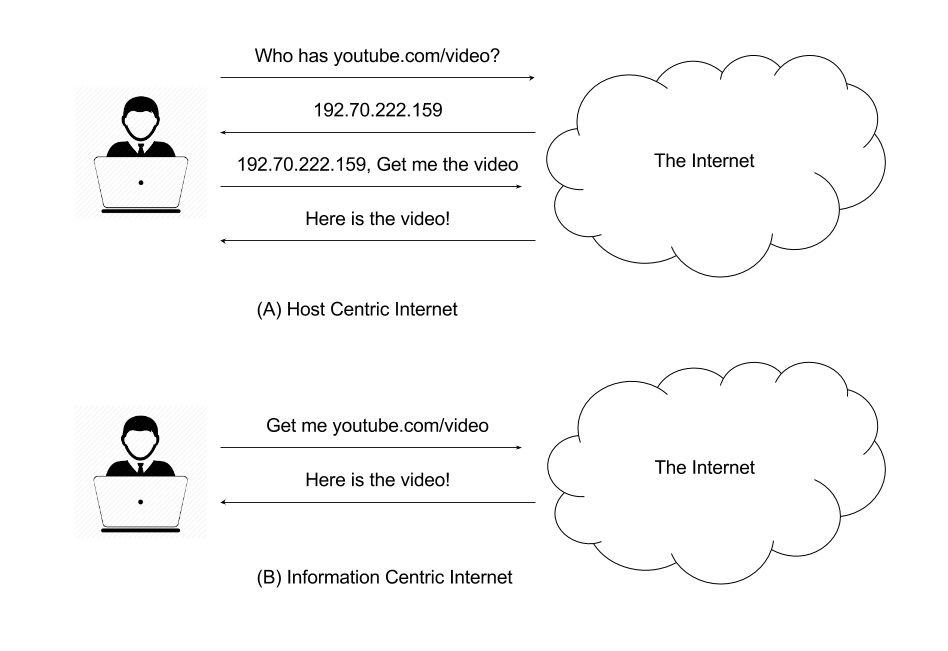
\includegraphics[scale = 0.5]{icn_illustration}
    \caption{Host Centric Internet vs Information Centric Internet}
    \label{fig:icn_illustration}
  \end{center}
\end{figure}

\section{eXpressive Internet Architecture (XIA)}
eXpressive Internet Architecture is a candidate future Internet
architecture that argues against elevating one particular
communication \emph{principal} type over others. A principal is a
named entity such as a host, a domain, a service or a specific content
piece. If the network primarily supports communication with one
particular principal type then communication with the other principal
type inherently becomes difficult. We see in today's host-centric
Internet that all the content requests first need to identify the host
who is capable of serving the content request. Similarly, if we moved
to an Information Centric Internet, it is not obvious how can we make
hosts communicate with each other. XIA, thus, supports coexistence of
multiple principal types.

Three key features of XIA are as follows:
\begin{itemize}
\item{Multiple Principal Types}
\item{Fallbacks}
\item{Intrinsic Security}
\end{itemize}
Let's go over these features one by one in order to understand XIA
better.
\subsection{Multiple Principal Types}
As seen above, XIA supports coexistence of multiple communication
principal types. The communication principals that XIA supports are
hosts, services, administrative domains and content. These principals
are identified by unique eXpressive identifiers called as
XIDs. Corresponding to the four principal types mentioned above, their
XIDs are referred to as HIDs, SIDs, ADs and CIDs.

\subsection{Intrinsic Security}
XIA's intrinsic security requirement mandates a communicating
principal to prove itself. In other words, it should be possible for
an entity that is communicating with a principal to verify the
authenticity and integrity of the principal. XIA, thus, chooses the
XID as such that they guarantee the authenticity and integrity of the
communicating principal. For example, the host identifier or the HID
is the secure hash of the host's public key. The content identifier or
the CID is the secure hash of the content itself.

\subsection{Fallbacks}
In order to support evolvibility, it becomes important to address the
issue of how network entities that do \emph{not} understand a
communication principal type deal with the principal. An analogous
example in today's Internet could be as follows. If we move to IPv6
Internet, what if an intermediate network does not understand IPv6 and
only understands IPv4? The intermediate nodes should not drop the IPv6
packets. In other words, the network still needs a way to forward
packets even if it does not understand a communication principal. XIA
supports this ability via the notion of fallbacks. Fallbacks allow XIA
to specify multiple paths to the same principal. The entities that do
not understand a particular path can take a different path for
communicating with the principal type. All the different paths to the
communication principal are combined into a network layer address that
takes the format of a directed acyclic graph (DAG) as shown in
\ref{fig:dag_address}. The address is interpreted as follows - forward
/ route primarily based on CID, but if you don't understand CID, route
based on IP address.

\begin{figure}
  \begin{center}
    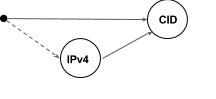
\includegraphics[scale = 0.75]{dag-cid-ipv4}
    \caption{Fallbacks}
    \label{fig:dag_address}
  \end{center}
\end{figure}

\section{Content Principal in XIA}
With the content principal users can express interest in content
irrespective of its location. Sending a content request fetches
content from anywhere in the network. The request could go all the way
back to the original publisher of the content or can be served from an
in-network cache that holds a copy of the content. The API for content
principal are as shown in table \ref{tab:cid_api}. Content principal
provides intrinsic security guarantees by choosing the cryptographic
hash of the content as its identifier. Thus, all the network devices
can verify authenticity of the content objects.

\begin{table}
  \begin{center}
    \begin{tabular}
      { l  p{3in} }
      Function & Description \\
      \hline
      getContent(socket, addr, buffer) & Retrieves the content specified
      by addr from network; addr contains CID and possibly a fallback \\
      putContent(socket, content) & Registers the content as
      available \\
      \hline
    \end{tabular}
    \caption{API for Content Principal}
  \end{center}
  \label{tab:cid_apis}
\end{table}

\section{Conclusion}
In this chapter, we studied the eXpressive Internet Architecture. We
looked at the importation features offered by XIA - coexistence of
multiple principal types, intrinsic security and fallbacks. Then we
looked at how network entities can use the content principal to
publish and fetch content irrespective of its physical location. This
was the last introductory chapter in the thesis. The following
chapters build on to ideas discussed in these two chapters and are the
main contributions of the thesis.
} % A regular chapter, starts with '\chapter{Title}'
\chapter{Content Retrieval Infrastructure}
\label{content_retrieval}

\section{Motivation}

Most of the applications today that need to deliver content reliably
use TCP as the transport layer protocol. The motivating example in our
case is the world wide web. TCP relies on communication from end-hosts
to provide reliable content delivery. Relying on end hosts rather than
the network for the reliable delivery information gives TCP the
advantage that no explicit network layer feedback is needed to
reliably transport content. This goes in accordance with the
philosophy of a dumb network and smart ends and the end-to-end
principle.

However, the rise of information centric networking shifts the focus
from hosts to content. That poses us with the challenge of redesigning
reliable transport for content centric architectures. The solutions
that have been proposed, rely on client applications to fetch
individual packets belonging to a object reliably. This approach of
one-way reliability loses on important congestion control information
that the content provider (a router cache or the original publisher)
could have received from the client. An example of such information
could be the congestion window size.

We, therefore, take a different approach to solve the problem of
reliable transport of content chunks. We use coexisting content and
service principals in XIA to allow us to apply TCP like congestion
control and reliability approach to content centric networks. The
content principal helps in locating the content and the service
principal helps in delivering the content. We show that this approach
of delivering content-over-service does not change the semantics of
use and still allows both the publisher and the client to
participate in a reliable content transport session resulting in a
more efficient reliable content transport for content centric
architectures.

\section{Design Goals}

As we have seen in the last chapters, XIA does not disregard the fact
that the first class principal the world is moving towards is
content. At the same time it allows for presence of multiple such
principals simultaneously. In the new content retrieval infrastructure
we aim to leverage the coexistence of service and content
principals. We aim to solve problem the problem of reliable transport
of content for content centric networks using the coexisting service
and content principals.

While solving other problems, we aim to ensure that the benefits
expected out of an information-centric architecture are still
preserved. So, ICN features such as on path caching, content based
routing should remain as they are.

Also, we envision that the cache on routers could extend in multiple
dimensions. For example, cache could choose to store content at a
remote location rather than in its local storage. Content eviction
policies might change over time.  Thus, it is important that the
system we design is extensible in all the ways possible.

To summarize, the goals of new content principal handling are as
follows:
\begin{itemize}
\item{Support Opportunistic Caching.}
\item{Support Reliable Transport for Content Objects.}
\item{Support Extensible.}
\end{itemize}
\section{Design Overview}

\begin{figure}
  \begin{center}
    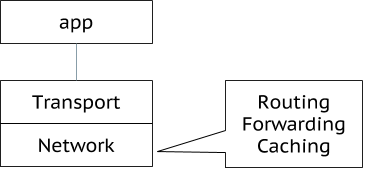
\includegraphics[scale = 0.75]{old_stack}
    \caption{Old Network Stack for Content Delivery Architecture}
    \label{fig:old_stack}
  \end{center}
\end{figure}

\begin{figure}
  \begin{center}
    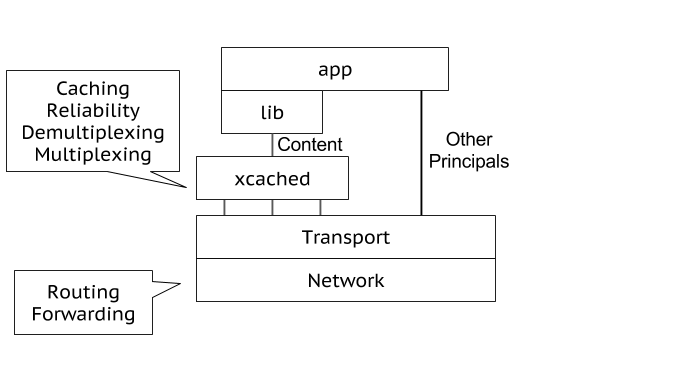
\includegraphics[scale = 0.75]{new_stack}
    \caption{New Network Stack for Content Delivery Architecture}
    \label{fig:new_stack}
  \end{center}
\end{figure}
As we have seen in chapter \ref{chap:ccnxia}, cacheable content is
addressed using CIDs. CID principal puts no limit on the size of the
content chunk. Although desirable, this requirement implies that some
applications will need the ability to transmit and fetch content
reliably. How does it affect our design?  Let’s look at where various
functionalities are implemented in XIA’s network stack. The old
network stack for content delivery architecture is outlined in
\ref{fig:old_stack}. Reliable transport service (streaming sockets) is
implemented at transport layer in this stack. In order to transmit
content reliably, we need a way to use reliable transport
service. Therefore in our new design, we implement content delivery
infrastructure primarily in an application while keeping content based
routing as it is. The new network stack and the functionality split is
as shown in \ref{fig:new_stack}.

The fact that caching is moved to an application gives us following
advantages:
\begin{itemize}
\item{Extensibility}
\item{Easy access to reliable transport API}
\end{itemize}

We define a new application level entity called Xcache Daemon(xcached)
that takes the responsibility of caching and serving content chunks.
Xcached receives requests from client applications and translates them
into socket calls as shown in \ref{tab:apis}. Xcached also takes
care of multiplexing and demultiplexing of content requests and
responses to and from various connected content applications.

\section{Xcached Architecture}

Xcached is the center of all CID (as well as nCID as we will see in
the later chapters) operations. So, it is important that it does not
become the bottleneck in the content delivery infrastructure. It
essentially means that xcached should not starve applications, it
should process requests fairly and it should be performant. In this
section we will look closely at the xcached daemon - how it has been
architected and what are some of its extensibility characteristics.

\begin{figure}
  \begin{center}
    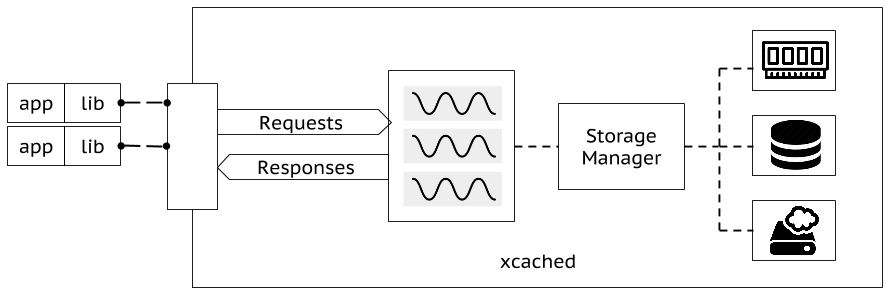
\includegraphics[scale = 0.45]{xcached_arch}
    \caption{Xcached Architecture}
    \label{fig:xcached_arch}
  \end{center}
\end{figure}
Xcached is a mutli-threaded program that follows worker thread pool
model in which the application facing controller puts the arrived
requests in a queue and worker threads dequeue and do the work as and
when convenient. \ref{fig:xcached_arch} shows the various modules in
the xcache daemon.

\subsection{XcacheLib}
In order to hide communication details from the application, we have
built a library that exposes the required APIs to the content
applications. These APIs are described in greater details in section
\ref{sec:apis}.

\subsection{The controller}
The controller is the application facing front end which takes
requests from the XcacheLib. The communication between the controller
and XcacheLib is over UNIX domain sockets. We use google-protobuf to
parse and unparse the requests to and from the controller. It is
possible that applications request for content that is cached
locally. The controller processes such requests in the
fast-path. I.e. It sends back the response to the application
quickly. All the other requests which cannot be processed in the fast
path are put in the requests queue. These requests are processed at
some time in future by one of threads in the thread pool.

\subsection{Thread Pool}
\begin{table}
  \begin{center}
    \begin{tabular}
      { p{1in} | p{2.5in} | cp{0.5in} |}
      Job & Details & No. of threads \\
      \hline
      Content Publish / Fetch & Storing content published by applications or fetching content from a remote source &  Arbitrary\\
      \hline
      Content Eviction on Timeout & Content objects that get cached have a associated time-to-live period. This is the time period after which content object should become unavailable. & One \\
      \hline
      Opportunistic Caching & Opportunistic caching of content chunks
      by in-network devices & One\\
    \end{tabular}
  \end{center}
  \caption{Jobs performed by threads in xcached}
  \label{tab:threads}
\end{table}
Xcached thread pool consists of a set of worker threads, number of
which can be configured at xcached startup. The thread pool consists
of threads that perform one of the tasks shown in \ref{tab:threads}.
\subsection{Content Stores}
Different content systems have different characteristics: RAM allows
fast retrieval of data but has limited size. Disk is slower than RAM
store but can hold a lot more content. Thus storing content in RAM
might be more desirable for use cases that need only smaller chunks
whereas use cases that need to store big content chunks might prefer
to store content on Disk rather than in RAM. In order to support these
varying use cases, Xcached supports multiple different content storage
methods. By default, it supports storing content in RAM, on disk and
on a network attached storage device. Also, it is possible to compile
new storage methods with xcached. Implementing a new storage method is
as simple as extending following class and implementing the member
methods.

{
  \setstretch{1.0}
\begin{verbatim}
class xcache_content_store {
        virtual store();
        virtual get();
}
\end{verbatim}
}

\subsection{Storage Manager}
Since xcached has different storage methods, it is possible to
organize content objects across these stores in different ways to
serve different use-cases. Possible content placement policies could
be round-robin, popularity based or size based. We implement a simple
content placement policy which places content in RAM store until it’s
full and then moves subsequent content to the disk store.

\subsection{Content Eviction}
If possible content stores run out of space, content must be evicted
to make space for new incoming content. Content eviction policies
govern which content chunks should be evicted on such an event from a
particular content store. The content eviction policy that Xcache
supports is LRU (Least recently used). Just like content stores, new
content eviction policies can be compiled with xcache and associated
with the content stores. Implementing new content store specific
content eviction policies is just as simple as extending and
implementing following class and associating it with a content store.

{
  \setstretch{1.0}
\begin{verbatim}
class xcache_eviction_policy {
        virtual store();
        virtual get();
        virtual remove();
        virtual evict();
}
\end{verbatim}
}


\section {Design Details}

Xcached has three types of interfaces with the transport layer. In
order to understand these interfaces better let's take a closer look
at three network components that interact with XcacheD.

\subsection{Content Server}
Xcached acts as a content server on the publisher's end as well as
when the in-network cache delivers content to the client. On receipt
of content requests, the daemon needs to know what content is being
requested. We define a new type of transport socket called ``content
server'' socket which allows daemon to bind to all the content
connections. This socket allows xcached to know for what content the
request was received.  The content server socket needs to do two
unusual tasks which are significantly different from normal server
sockets.

\subsubsection{Bind(Content *)}
Since content server needs to listen to all incoming content
request, it needs to bind to all content addresses that the provider
has with it. Thus we need a notion of \texttt{Bind(Content *)}.

\subsubsection{AcceptAs(MyAddress)}
As the server side socket has been bound to many addresses, when an
incoming request is received, the xcached needs to know for which
address the request was received. In other words, the server needs a
way to know what address is the source address for packets going out
of it. Thus we define a new \texttt{AcceptAs} call that tells xcached
for which content the request was received.

\subsection{Content Client}
The main responsibility of client side xcached is to establish a
reliable transport session with a content provider and fetch content
reliably. The content provider can be an in-network cache or it can be
the end publisher. So, xcached's client side socket ``connects'' with a
content provider and fetches the content. In other words, xcached's
client socket ``connects'' with content rather than a ``service''.

\subsection{Opportunistic Caching}
The last context in which xcached comes into picture is opportunistic
caching. When content providers serve content to clients over a
reliable transport session, in-network devices need to intercept and
cache content packets as they are traveling through them. The third
interface that xcached has with the network allows xcached to sniff
content packets flowing through it. We call this socket a content raw
socket.

\begin{table}
  \begin{center}
    \begin{tabular}
      {| c | c |}
      API & What xcache does \\
      \hline
      XputChunk & StoreContent(), XaddRoute() \\
      XgetChunk & Xconnect(CID Dag), Xrecv() \\
    \end{tabular}
  \end{center}
  \caption{API Expansion}
  \label{tab:apis}
\end{table}
\section{End to End Example}

We have seen at high level how we moved caching and content serving
functionality to xcached application. In this section we will walk
through a detailed end to end example and see how clients establish
a reliable transport session with a publisher and how intermediate
caches cache the packets flowing through them.

\subsection{Step 1: \texttt{XputChunk(Content)}}
The whole story starts with the publisher putting the content objects
in the local cache (xcached) and publishing routes to these content
objects. This lets the network know that unless cached at a better
location, all the incoming requests for this content should be
forwarded to this host. The end publisher publishes the chunk with the
DAG address as shown in \ref{fig:cid_dag_publisher}.

\begin{figure}
  \begin{center}
    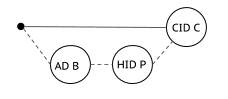
\includegraphics[scale = 0.75]{cid_dag_publisher}
    \caption{CID Dag Publisher}
    \label{fig:cid_dag_publisher}
  \end{center}
\end{figure}
\subsection{Step 2: \texttt{XgetChunk(CID\_Dag)}}
\begin{itemize}
\item{Client application calls \texttt{XgetChunk} with the desired DAG
  address as the argument. This call lets the xcached know that a client
  application is interested in fetching content pointed to by the
  DAG.}
\item{Xcached tries to establish the reliable transport session with
  one of the many network entities who can serve the content by calling
  \texttt{Xconnect(CID-Dag)}. This \texttt{Xconnect(CID-Dag)} call
  serves two purposes: It acts as a content request as well the first
  packet of three-way handshake of the reliable transport session
  (SYN).}
\item{Any network device that has the content chunk cached, accepts
  the GET / SYN packet and in effect tells xcached that there is a
  content request and it is the first packet of the reliable transport
  session.}
\item{Call to \texttt{XacceptAs} made by xcached then returns with the
  address of content that was requested by the client. Calling
  \texttt{XacceptAs} results in generation of SYN-ACK. The return of
  \texttt{XacceptAs} also means that the three-way handshake was
  completed by the xcached that provides the content.}
\end{itemize}
\subsection{Addresses}
The SYN packet that xcached on the content provider received, has the
source address that looks like address in \ref{fig:dag_syn_source}.

\begin{figure}
  \begin{center}
    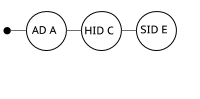
\includegraphics[scale = 0.75]{dag_syn_source}
    \caption{SYN Source Address}
    \label{fig:dag_syn_source}
  \end{center}
\end{figure}
The SID in the source address represents the ephemeral reliable
transport endpoint that xcached on client had created. This address
acts as a way back to the client. Content server socket completes
the three way handshake by accepting the connection with source
address as in \ref{fig:source_cid_addr}.
\begin{figure}
  \begin{center}
    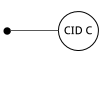
\includegraphics[scale = 0.75]{cid_dag_published_chunk}
    \caption{Published Content Chunk Address}
    \label{fig:source_cid_addr}
  \end{center}
\end{figure}
Once the connection has been accepted, content provider serves the
content over the established reliable transport session.

\subsection{Opportunistic Caching}
The challenge in opportunistically caching the content objects is that
the xcached on the in-network cache is not an active participant in
the reliable transport session. We solve the problem of opportunistic
caching by forwarding all the content packets to xcached and then
reassembling the chunk by peeking into transport header. Following are
the steps that take place on the intermediate cache when content
object is to be cached.
\begin{itemize}
\item {While content is being served from the content provider to content
client, it gets caught by the CID raw sockets on Xcached's running
on intermediate network devices. The CID raw socket forwards all the
packets which have the primary intent as CID to the xcached
running.}
\item {Looking at the first packet in the transport session (SYN/ACK),
  the forwarding engine needs to know if the content object should be
  cached or not. The logic for this policy is implemented in
  xcached. Based on the policy, xcached takes a decision and either
  sends ``Yes, cache'' or ``No, don't cache'' decision to the
  forwarding engine}
\item {Packets belonging to all content chunks for which the policy
  decision is ``Yes, cache'' are forwarded to xcached.}
\item {Xcached peeks into the transport header and reassembles a
  content object. Once reassembled, now that particular xcached also
  acts as the content provider for the chunk.}
\end{itemize}


\section{API Details}
\label{sec:apis}
With the movement of caching and content handling to xcache
application, we also redefined the application interfaces for
publishing and fetching content over XIA. The application is not
responsible for establishing the reliable transport session. Xcached
does it on behalf of the application. This simplifies the application
design and also gives the xcached the ability to cache content that
was requested by the application. In this section, we will go over the
APIs that XcacheLib exposes to the content applications and see an
example of a sample content publisher as well as a client application.
\begin{itemize}
\item{\texttt{int XcacheHandleInit(XcacheHandle *h)}} - Creates a
  connection with \texttt{xcached} and fills in the opaque structure
  \texttt{XcacheHandle}. \texttt{XcacheHandle} acts as a context for
  the rest of the APIs.
\item{\texttt{int XcacheHandleDestroy(XcacheHandle *h)}} - Destroys
  the the handle created by the call
  \texttt{XcacheHandleInit}. Applications that call
  \texttt{XcacheHandleInit} must call \texttt{XcacheHandleDestroy}.
\item{\texttt{int XfetchChunk(XcacheHandle *h, void *buf, size\_t buflen,
    int flags, sockaddr\_x *addr, socklen\_t addrlen)}} - This
  function lets applications fetch content chunk that has the DAG
  address \texttt{addr} of length \texttt{addrlen}. The Xcache context
  \texttt{h} must be initialized by calling function
  \texttt{XcacheHandleInit}.

\item{\texttt{int XputChunk(XcacheHandle *h, const void *data, size\_t
  length, \\sockaddr\_x *addr)}} - \texttt{XputChunk} allows
  applications to publish chunks to the network. A call to
  \texttt{XputChunk} publishes a chunk which has data pointed to by
  \texttt{data} and of length \texttt{length}. The address of the
  published chunk is returned in the address \texttt{addr}.
\item{\texttt{int XregisterNotif(int event, \\void (*func)(XcacheHandle
    *, int event, sockaddr\_x *addr, socklen\_t addrlen))}} - Xcache
  allows applications to listen for certain
  ``notifications''. Examples of these notifications include chunk
  eviction notification, chunk arrival notification. A call to
  \texttt{XregisterNotif} registers a handler for a particular
  notification. Applications can either spawn a separate thread for
  handling notifications by calling \texttt{XlaunchNotifThread} or
  they can look for received notifications by checking received data
  on socket returned by \texttt{XgetNotifSocket} and calling
  \texttt{XprocessNotif} if appropriate.
\item{\texttt{int XlaunchNotifThread(XcacheHandle *h)}} - This
  function launches a notification listener thread. If
  \texttt{xcached} sends a notification on notification socket, the
  function calls registered handlers if appropriate.
\item{\texttt{int XgetNotifSocket(XcacheHandle *h)}} - This function
  returns the socket on which \texttt{xcached} sends back the
  notifications.
\item{\texttt{int XprocessNotif(XcacheHandle *h)}} - If the
  \texttt{xcached} notifcation socket has any incoming data,
  applications can call \texttt{XprocessNotif} to invoke the
  registered handlers.
\end{itemize}

\section{Sample Applications}
In this section, we will see how applications can use above mentioned
APIs in their code. Section \ref{sec:content_server_app} shows a
self-explanatory example of a content server application. Whereas,
section \ref{sec:content_client_app} shows a self-explanatory example
of a content client application.

\subsection{Content Server Application}
\label{sec:content_server_app}
      {
        \setstretch{1.0}
\begin{verbatim}
  int main(void) {
    XcacheHandle xcache;
    sockaddr_x info;
    ...
    XcacheHandleInit(&xcache);
    ...
    XputChunk(&xcache, data, datalen, 512, &info);
    ...
    XdetroyChunk(&xcache);
  }
\end{verbatim}
      }

\subsection{Content Client Application}
\label{sec:content_client_app}
      {
        \setstretch{1.0}
\begin{verbatim}
  int main(void) {
    XcacheHandle xcache;
    sockaddr_x info;
    ...
    XcacheHandleInit(&xcache);
    ...
    XfetchChunk(&xcache, buf, 1024, XCF_BLOCK, &info, sizeof(sockaddr_x));
    ...
    XdetroyChunk(&xcache);
  }
\end{verbatim}
}
\section{Conclusion}
In this chapter, we saw how we moved content caching and serving to an
application daemon \texttt{xcached}. In contrast to the old design, we
used reliable transport to deliver content. We then looked at the new
API and how we can use it to write content applications in XIA.
}
\chapter{Fetching Named Content in XIA}
\label{chap:namedcontent}

\section{Motivation}

In order to effectively utilize in-network caches, it is important
that the resources in the web are cacheable. Cacheability of the
resources really depends on its reusability. Static resources (objects
images, video chunks) are probably the best candidates for utilizing
in-network storage. But, the majority of web content falls in the
other two categories.

It can be argued that dynamic resources can benefit the least from of
in-network caches. The primary reason being that dynamic resources are
generated upon the request arrival and hence are highly
non-reusable. This, clients can thus

But the resources that are of interest to us are the multiform
resources that we saw in chapter \ref{chap:www}. Recall that these
resources exist in multiple forms at a same time or at different
times. Clients \emph{choose} a representation that suites their need
the best. They are reusable for the very reason that upon sending the
same request multiple times, they respond with the same content. What
can we do to make these multiform resources cacheable at the same time
preserve their multiformity?

\subsection{Human Readable Names for Multiform Resources}

We have seen that web relies on human readable names for identifying
multiform resources and in general all the web resources. Even though
cryptographic identifiers have inherent security properties, what
makes human readable names a preferred choice?

The first obvious reason is that the names are more
understandable. Users establish trust in human readable Identifiers
such as``facebook.com'' much easily than in random cryptic hex string
such as ``0ABF1866BD7182...''.

The second reason is that multiform resources change their
representation. For example, content associated with the resource
identified by ``http://www.cnn.com'' changes often. So, as time passes
multiform web resources change their representation. Also, time is not
the only dimension along which these resources change their
representation. Another such dimension could be UserAgent. With the
advent of smart-devices, number of platforms from which web resources
are accessed has been increasing like never before. That poses us with
the challenge of presenting the same resource in different forms based
on the platform that the user is requesting the resource from.

CIDs have the disadvantage that an identifier can only point to a
particular representation. It also implies that it is not possible for
us to allocate an identifier for content that we don’t know in
advance. So, crypto IDs do not support the property of late binding.

\section{Locating Content using Human Readable Names}

In the last section we saw the reasons why the world wide web
identifies and locates resources by human readable names. Let’s see
the possible options to locate content using human readable names in
eXpressive Internet Architecture.

\begin{itemize}
\item Keep a DNS like mapping system that maps names to CIDs
\item Locate content directly by human readable names
\end{itemize}

\subsection{Problems with DNS like mapping system}

In this approach, we would need a naming system that maps human
readable names to CIDs. Users first query the naming system to get the
CID and then request the CID. The naming systems could well be
established at organizational levels like today. Although scalable,
this approach suffers from following issues.

Size of the mapping system: Firstly, the size of the mappings that the
system needs to maintain is directly proportional to number of
cacheable objects that the publisher has as opposed to number of hosts
in today’s Internet. It is evident that number of objects outnumbers
number of hosts by orders of magnitude. So, we would need really huge
mapping system.

Number of roundtrips: In order to fetch a CID for a particular name,
the web user would need to make several roundtrips to and from the
naming system. Depending upon the model used by the naming system, the
consumer could take from one to several roundtrips before it can know
the CID corresponding to the content name.

Security Issues: Once the consumer receives CID corresponding to a
human readable name why would the consumer believe that mapping
between the human readable name and the CID is authentic? Hence, the
content retrieval architecture must address these security issues
somewhere. However, that loses the whole point of having cryptographic
identifiers. Remember that one important property of CIDs is that they
are self certifying.

Because of the issues mentioned above, it becomes unwise to use a
naming system for locating content by name. Therefore, we take the
second approach of directly addressing content by human readable
identifiers. The following sections describe the new principal type
that we define and address the security concerns raised by human
readable names.

\section{nCID Principal Type}

\subsection{Definition}

In order to effectively eliminate a huge naming system and support the
multiform content on the world wide web, we define a new principal
type which allows locating content directly by human readable
names. Just like CIDs, the content requested by the consumer using
nCID is retrieved from anywhere in the network. The XID type nCID is
defined as follows:

\begin{verbatim}
nCID = hash(Human Readable Name + Publisher's Public Key Fingerprint)
\end{verbatim}
nCID is thus content with a human readable name that is verified by a
publisher.

\subsection{Semantics}

\begin{table}
  \begin{center}
    \begin{tabular}
      {p{2in}  p{3in}}
      API & Details \\
      \hline
      XputNamedContent(Buffer, Name, Certificate, Signature) &
      Publishes a named content chunk with the corresponding signature
      and the certificate\\
      XgetNamedChunk(Name, Certificate) & Fetches a name content chunk
      and verifies the authenticity and integrity using the public key
      certificate\\
    \end{tabular}
  \end{center}
  \caption{nCID Principal Semantics}
  \label{tab:ncidapis}

\end{table}

The nCID principal allows users to retrieve content identified by
human readable names from anywhere in the network. \ref{tab:ncidapis}
shows the APIs that nCID supports. Similar to CIDs, sending content
request for nCID type using \texttt{getNamedContent()} initiates a
transport session with any in-network cache or the original
publisher. This reliable transport session is then used to deliver
content to end consumers.

The \texttt{publishNamedContent(name, signature, public key
  fingerprint)} call tells the network that the content identified by
a human readable name is available with the publisher. It is verified
by a private key corresponding to the public key passed as an
argument. Xcache expects that the signature passed an argument is
generated in a certain way (we elaborate upon it in the following
section). The public key fingerprint and the signature is used by
in-network devices and the endpoints to perform security checks.

\section{Security Issues with Named Content}

\subsection{nCID Security Requirements}

XIA’s intrinsic security requirement makes it mandatory for the XIA
prinicpals to provide integrity and authenticity for the communication
operation. CIDs provide the integrity and authentication by defining
identifiers as the hash of the content so that when the consumer
receives the content and the CID, it has a reason to believe that the
content has not be tampered with and has been received from an
authentic publisher.

We argue that satisfying following four requirements provides exactly
these guarantees for nCID principal type.

\begin{enumerate}
\item{Ability to Verify Binding between Name and Content} \\
The consumer and in-network devices should have a reason to believe
that the content and name are tied together. CIDs provide this
guarantee inherently. For nCIDs, we rely on public key infrastructure
to provide the guarantees.
\item{Ability to Verify Content Integrity} \\
The consumer should have a reason to believe that the content has not
been tampered with.
\item{Ability for Caches to Verify All These at Minimum Cost}\\
The in-network caches need to perform these security checks before
they can cache a copy of the object. Applications can use different
trust models. It would be inefficient for in-network caches to verify
authenticity, integrity properties of the content chunk based on the
application specific trust model. So, we need an application agnostic
security model to work with.
\item{Protection against Content Poisoning} \\
Since there is no absolute binding between the name and the content,
an attacker can claim that certain content can belong to a particular
name. Our security model must prevent such an action.
\end{enumerate}
\subsection{Security Model}

Previous work argues that in order to provide security guarantees it
is sufficient to bind any two pairs between name, content and
publisher. We choose to bind name-content and name-publisher pairs.

In order to understand how our security model functions let us look at
some important chunk headers that nCID chunk contains.

\begin{figure}
  \begin{center}
    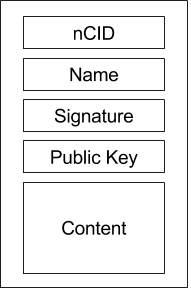
\includegraphics[scale = 0.75]{ncid_chunk_structure}
    \caption{nCID Content Chunk Structure}
    \label{fig:ncid_chunk_structure}
  \end{center}
\end{figure}

Name-content binding is provided by the digital signature that the
publisher generates at publish time. Name-publisher binding is
provided by the nCID itself. Following equations show how these
bindings are created by the publisher.
\begin{center}
\texttt{\textbf{nCID = hash(Content Name, Publisher's Public Key Fingerprint)}}\\
\texttt{\textbf{Signature = Encrpyt\_with\_Publisher's\_Private\_Key (Content Name, Content Data)}}\\
\end{center}
As long as the consumer knows about the name of the content and the
original publisher's public key fingerprint, it can always generate a
content request. So, we expect that some high level entity (such as a
TLS connection) delivers these two parameters to the end consumer. In
the next chapter about URLs, we see how sophisticated URLs for nCID
can be used to serve this information.

nCID intrinsic security checking is a two-step process in contrast to
one-step process in case of CIDs. The entity that needs to verify
authenticity and integrity of the content chunk must first fetch the
public key that was used to verify the content. The content chunk
contains a pointer to the public key chunk.

Once the public key has been received, the consumer checks if nCID
matches the hash of name and publisher’s public key fingerprint. It
then decrypts the signature with the same public key. The decrypted
signature is matched against name-content pair. If both these checks
succeed, then consumer can safely believe that content is authentic
and has not been tampered with.

No matter what trust model the application uses, all the in-network
devices need to perform only one public key fetch and the two checks
for nCID and signature. Thus, the time required for verifying security
properties is constant. Besides, it requires at most only one content
chunk fetch. This satisfies our third requirement of verifying
security properties at minimum cost.

\subsection{Protection against Content Poisoning}
Content poisoning is an attack in which the attacker claims that a
certain malicious content belongs to certain name that has already
been published in the network. \ref{fig:content_poisoning} shows the
motivating example.

\begin{figure}
  \begin{center}
    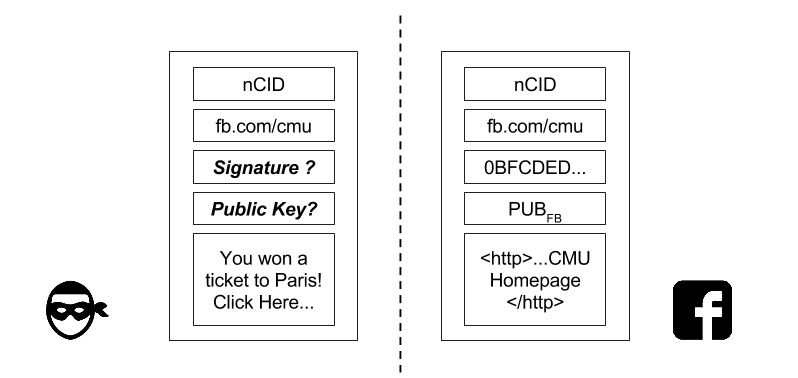
\includegraphics[scale=0.5]{content_poisoning}
  \caption{Content Poisoning}
  \label{fig:content_poisoning}
  \end{center}
\end{figure}

In this example, the original publisher facebook.com has published a
nCID chunk named ``fb.com/cmu''. Facebook has verified the chunk and
put its signature in the chunk header. Now, an attacker wants to claim
that certain spoofed content actually belongs to the name
fb.com/cmu. What possible options he has to fill in signature and the
public key?

\begin{itemize}

\item{\textbf{Option 1: Public Key = Facebook’s Public Key}} \\
If attacker uses facebook’s public key itself then he cannot generate
the corresponding signature. So, this option is not really possible.

\item{\textbf{Option 2: Use my own key}}\\
Let’s say the attacker uses his own key to generate the signature. In
that case, even though attacker successfully plants a spoofed
signature in the chunk he breaks the nCID check.

\end{itemize}

So we have seen that the attacker has no way of successfully filling
in the signature and public key field pairs. Content poisoning is thus
not possible in our security model.

\section{Conclusion}
We defined a new content principal for XIA that allows us to directly
address the content by human readable names. We argued that such a
principal best suites the ``multiform web resources''. However, such a
content addressing system faces the issue of content authenticity and
content integrity. We defined security models that address these
authenticity and integrity issues to provide us an alternate secure
content principal.
}
\chapter{URLs for Content in eXpressive Internet Architecture}
\label{sec:urls}

\section{Universal Resource Locators (URLs)}
The resources in the world wide web are identified by
\textbf{Universal Resource Identifier} often acronymed as
\textbf{URIs}. URIs allow identifying resources uniquely thus giving
hosts the ability to express interest in specific resources. The most
common form of URIs is \textbf{Universal Resource Locators or
  URLs}. URLs, in addition to uniquely identifying a resource also
specifies a mechanism to retrieve the resource. The URLs in general
look like the following:

\begin{center}
  \textbf{\textit{protocol}://\textit{host}/\textit{path}}
\end{center}

The \textit{protocol} field specifies the scheme that should be used
to retrieve a representation of the resource. The most popular
resource retrieval scheme in the web is `HTTP'. Other possible schemes
are `FTP', `file', `data'. The \textit{host} part is the network
location of the resource. It can be an IPv4 address or a domain name
that the DNS can resolve to an IPv4 address. A \textit{host} can own
multiple resources. The \textit{path} is the specific location of the
resource on the \textit{host}.

\section{URL Design Goal}
The goals of URL design for CIDs and nCIDs are two-fold.

Firstly, the web resources refer to other web resources all the
time. For example, the HTML web pages contain URLs of other web
resources. In the previous chapters we have seen that the CIDs can be
used better to represent static web resources. On the other hand,
nCIDs are a better fit for multiform resources. Since, in this thesis
we use CIDs and nCIDs to represent web resources, we need a method of
pointing to these web resources.

Secondly, the advantage that nCIDs have over the CIDs is that they are
addressable by human readable names. Hence, constructing nCID URLs is
a fairly understood problem. But the goal of URL design for CIDs is
that the constructed URLs should be able to directly refer to the
content avoiding name lookups.


\section{URLs for CIDs}
\label{sec:urlcid}
We propose following format for CID URLs.
\begin{center}
  \textbf{\textit{cid}://\textit{serialized-cid-dag}}
\end{center}
In order to understand the process of DAG serialization, let us take
an example of a CID DAG address as shown in \ref{fig:cid_dag}.

\begin{figure}
  \begin{center}
    \label{fig:cid_dag}
    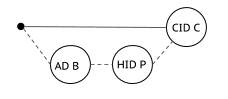
\includegraphics[scale = 0.75]{cid_dag_publisher}
    \caption{An example CID DAG address}
  \end{center}
\end{figure}

We follow the following process to make a serialized version of the
DAG:
\begin{enumerate}
  \item{Number all the nodes starting with zero and excluding the
    source node.}
  \item{List all the nodes in the order they are numbered from zero to
    maximum.}
  \item{For each node, associate the destination node number for all
    the \textit{outgoing} edges from that node.}
  \item{Prepend the output of the last step with the outgoing edges
    from the source node.}
\end{enumerate}

\begin{figure}
  \begin{center}
  \label{fig:cid_dag_serialization}
  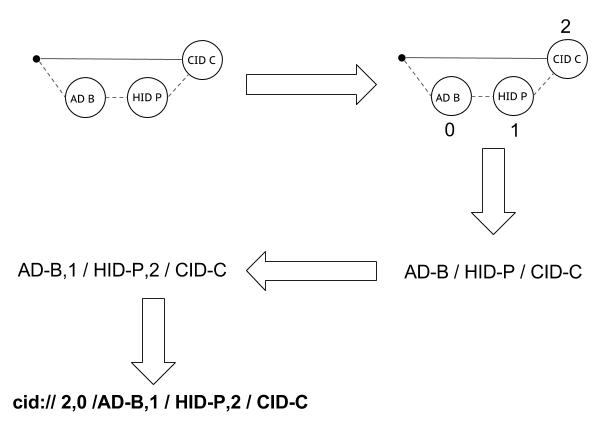
\includegraphics[scale=0.75]{dag_serialization}
  \caption{CID DAG Serialization}
  \end{center}
\end{figure}

This scheme results in an URL for CIDs that looks like this
\begin{center}
  \textbf{cid://2,0/AD-B,1/HID-P,2/CID-C}
\end{center}
The URLs that are created by this scheme are highly expressive. You
can see that \emph{any} DAG can be expressed by this method. That
allows us to use protocols other than CIDs too. For example, we could
create an URL for representing a service S as follows.
\begin{center}
  \textbf{\emph{sid}://2,0/AD-B,1/HID-P,2/\emph{SID}-S}
\end{center}
These URLs, since they directly address the content, avoid name lookup
completely. With these URLs we can now represent static resources in
the web.

\section{URLs for nCIDs}
We could readily use the URL scheme that we discussed in section
\ref{sec:urlcid}. But, the disadvantage of such an approach is that
the URLs created are highly unreadable. Since nCIDs are directly
derived from human readable names, we define a URL scheme which
results in URLs as we see today and yet avoids the need of name
look-ups completely.

\subsection{Addresses and Locators}
\label{sec:addrnloc}
We have seen that nCIDs are most useful for representing the multiform
web resources. The peculiar characteristic of multiform resources is
that they change their form based on certain \emph{attributes}. In
essence, all the representations of the same resource share the same
\emph{address} but are uniquely identified when the address is coupled
with the \emph{attributes}. We call the attributes that locate a
certain representation of a resource the \emph{locators}.\\
As a motivating example, let's take a case of multiform resources
identified by URL \emph{http://wikipedia.org/google}. It is easy to
see that when this web resource is requested from a desktop it takes a
certain representation. While the same resource, if requested from a
mobile device, takes a completely different form. So, even though the
two objects are totally different in terms of their content, they do
share an identity. This identity is their address. To sum up,
address of a multiform resource allows us to identify a resource and
locators help us locate a representation of the resource.

\begin{figure}
\begin{center}
  \label{fig:multiform-change}
  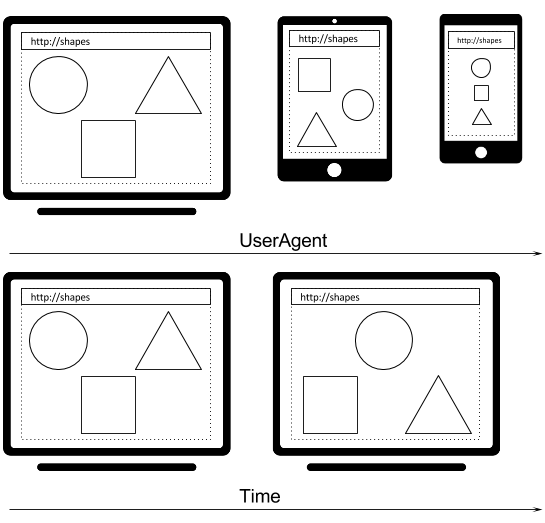
\includegraphics[scale=0.75]{multiform_changing_form}
  \caption{Multiform resource changing its form}
\end{center}
\end{figure}

\subsection{nCID URL Design}
Based on the learning from section \ref{sec:addrnloc}, we propose the
following format for the URLs of nCIDs.
\begin{center}
  \textbf{ncid://address/locator1=value1\&locator2=value2\&...}
\end{center}
With respect to the motivating example shown in figure
\ref{fig:multiform-change}, the address of the content is
\emph{content.facebook.com} whereas an locator is
\emph{UserAgent=Android}. Table \ref{tab:locators} shows the list of
possible locators. Our security model enforces us to mandate either
the implicit or the explicit existence of a locator called
\emph{certificate}. The locator \emph{certificate} is essentially the
pointer to the public key certificate that would be used to verify
authenticity and integrity of the named content chunk.

\begin{table}
  \begin{center}
    \begin{tabular}
      {c | c | c}
      Name & Details & Mandatory \\
      \hline
      PubCert & DAG Address of the Publisher's Public Key Certificate & Yes \\
      Version & Version of the Content Chunk & No\\
      UserAgent & HTTP UserAgent & No\\
    \end{tabular}
    \label{tab:locators}
  \end{center}
  \caption{List of Locators}
\end{table}

\section{Conclusion}

In this chapter, we defined URL schemes for CID and nCID type content
chunks. With CID URLs, we provided a way to point to CID chunks while
avoiding name lookups. The nCID URL scheme allows us effectively
express a link to a nCID resource. Separating addresses and locators
gives web users the ability to choose specifically the representation
that suites its needs the best.

}
\chapter{Conclusion}
\label{sec:conclusion}

The old implementation of the content principal did not support
reliable transport of content objects. The ability to reliably deliver
content objects is crucial for the World Wide Web. We thus implemented
content principal implementation to an application called
XcacheD. Moving content principal implementation to an application was
not a trivial task. It involved redefining interfaces with the network
stack. We carefully studied possible approaches and implemented the
content principal handling in Xcached application.

In order to fetch content objects directly by human readable names, we
defined a new XIA principal type - nCID. We addressed the authenticity
and integrity issues of the new principal type. The new principal type
allowed the clients to avoid name lookups for fetching content chunks.

We classified the web resources into three categories: static
resources, dynamic resources and multiform resources. XIA's different
communication principals supported these different web resources. We
argued that the static resources can be well represented with CIDs,
the dynamic resources can be well represented with SIDs and the
multiform resources can be well represented with nCIDs.

In order to effectively reference these various resources, we defined
a URL scheme. We defined a generic URL scheme to map any XIA address
to serialized character string. This scheme allowed us to represent
addresses of static and dynamic resources. We then defined URL format
for nCID principal that allowed us to address the multiform resources.

With the above contributions, we modeled the World Wide Web on
eXpressive Internet Architecture.
}

%==============================================================================

%-----------------------------------------------------------------------------%
% BIBLIOGRAPHY -- uncomment \nocite{*} to include items in 'mybib.bib' file
% that aren't cited in the text.  Change the style to match your
% discipline's standards.  Of course, if your bibliography file isn't called
% 'mybib.bib' you might want to change that here too :)
%-----------------------------------------------------------------------------%
\nocite{*}
%\bibliographystyle{./Bibliography/jasa} %Formats bibliography
\bibliographystyle{./Bibliography/IEEEtranS} %Formats bibliography
\cleardoublepage
\normalbaselines %Fixes spacing of bibliography
\addcontentsline{toc}{chapter}{Bibliography} %adds Bibliography to your table of contents
\bibliography{./Bibliography/References} %your bibliography file - change the path if needed

%-----------------------------------------------------------------------------%
% APPENDICES -- OPTIONAL. These are just chapters enumerated by Appendix 1,
%                Appendix 2, Appendix 3...
%-----------------------------------------------------------------------------%
%\appendix
%\chapter{Populo Ornatus}

Ut quando convenire scripserit mei, ut accusam noluisse eam. At scripta democritum quo, reque everti an qui, posidonium efficiendi ut mel. Pro an reque habemus, augue nemore conceptam in vim. Eu cibo ancillae takimata usu.

No vis albucius rationibus, eum doming ceteros constituto id. Ad suas zzril laudem cum. Natum mollis singulis vel te, ea elit imperdiet duo, odio inermis et eos. Nam ad vocibus tractatos, sit no vidisse diceret omnesque, mollis omnesque ea mea.

Ut est ridens principes scribentur, menandri interesset adversarium ius ut. Ut duo elit dissentias, at sea eleifend scripserit, eam nibh rebum definitiones an. Cum te quaeque epicuri mentitum, his elitr essent et, in sea habeo aliquid convenire. Quo euismod sadipscing definitionem an, ut duo iusto aliquando, graece appetere ne nec.

Consul imperdiet dignissim vis et, mei liber vidisse principes et, eu nam docendi voluptua democritum. Qui no dicat tamquam sanctus, saepe tincidunt no mel. Pro ignota albucius consetetur in, sint qualisque assueverit eam ut, vis graeco denique signiferumque ne. Sale appellantur contentiones eu his, pro magna ornatus ut, ad vidit omnesque euripidis pri. Sea congue moderatius in, his dicit suscipit no, mei ei incorrupte assueverit. Nusquam nominavi et quo, idque delenit vim an, posse quaeque an mea.

Suas elitr lucilius sit an, aeterno persius vel eu. Mel at essent aperiam repudiare. Tale consul eum ne, eam no meis delenit iudicabit, an sint mutat pri. Nec no clita propriae pericula, duo explicari gubergren ei. Ne sit autem nominavi, te falli deserunt per. Quo tractatos suscipiantur ex, electram dignissim usu no, cu congue iriure vivendo vim.

At vero graeci fuisset his, quo similique persequeris ad. Ex est graece mandamus, antiopam voluptatum his ea. Assum appellantur mel an, ei mea veri commune efficiendi. Pri blandit urbanitas no. Nam ex enim reque, ut nec iusto regione ullamcorper, facer harum pertinacia mei ei. Erant veniam imperdiet an eam, veniam mucius equidem ius eu, at scripta labitur est.

Et quo soluta graecis accommodare. Tamquam mentitum menandri vim ut. Ut nec melius senserit, ut mei sale aeque. Prompta delectus mea te, fierent adipisci ad per, mei odio pertinax senserit et. Per ut persius singulis. Id qui malorum iracundia, semper conceptam cu sed.

Vis nominavi urbanitas intellegat an, ut numquam deseruisse sea. Et quo dico aeque adipiscing, ius ea commodo epicurei, eum cu nulla imperdiet efficiantur. Ea cum simul scripserit. Ius reque decore voluptaria ei, nec sensibus mediocrem eu, sit iriure vivendo ad. At munere maiestatis mel, ex persius honestatis nec. Nihil omnes definiebas duo cu, dicat ancillae no vix. No est prompta apeirian, mel ad quaestio theophrastus mediocritatem.

Persequeris intellegebat disputationi et nec, nam ne alia solum reque, ad pri clita appellantur reprehendunt. Clita iracundia ex cum, placerat invidunt dissentias ius id. Possit dictas recteque sed ne. At eam singulis recusabo intellegat, ius in probo clita posidonium, id atqui paulo rationibus pro. Ut elit mucius qui. Mel ea ubique nostrud takimata. Cu eos vituperatoribus temporibus feugait.

Per putent nusquam oportere cu, nullam discere te sea, an vix quot mutat. Cibo reque nostrum nec eu, justo mucius aeterno vis id. Facer tempor cu vix, ex saepe similique maiestatis qui, ne pro eripuit offendit. Id mel cetero efficiantur. Cum homero aeterno euismod an, vulputate definitiones ne quo.

Sed exerci incorrupte et, usu mundi molestiae reformidans in, at probo vocibus quo. Ex vel aliquip maluisset. Qui enim error an, molestie incorrupte an ius. Id maiestatis temporibus mei, tantas oporteat ocurreret id pri. Ei nam velit doming utroque.

Suas vituperata mel eu, ex veri omnes duo, an modo molestie ius. At vis moderatius dissentias scripserit, nullam aliquam usu no. Cibo diceret sed an. Sea cu ridens convenire.

Pro prima blandit no. His ut dicit iriure oblique, eos meis urbanitas abhorreant te. Usu cu perpetua principes. Mutat utinam insolens id cum. Quo tale iudicabit conclusionemque ex. Eos id harum accommodare.

Vel legere liberavisse ut, et aeque timeam usu. Vis eu dico sanctus appetere, id vix graecis repudiare, ad persecuti mnesarchum mei. No atqui nemore deseruisse eum. Meliore accumsan accommodare in qui, an tation rationibus has, ea nulla aliquip euismod his.

Utinam ridens cum eu. Duo aliquam omnesque cu, sea elitr appetere ea. Mea no quas discere apeirian, munere hendrerit conceptam duo an, nec ad habeo tritani. Vis exerci volumus no. Omittantur reprehendunt no has. Malis accusata necessitatibus no nam.

No solet assentior ius, an ferri dissentiet pro, vix ad tantas offendit. Pro tollit consequat gloriatur ne, eu vix amet posidonium. Errem utamur veritus vix ea. Sed laboramus omittantur id, ut sonet voluptatum has, cu doctus iriure menandri eos.

Regione iudicabit ei per. Cum ea aliquip voluptatibus. Sit in partem explicari. Ne probo labores placerat mei. Ullum pertinax ea his, per cu persius impedit adipisci. Fabulas ancillae dignissim ei his, ius no nulla melius suscipiantur, ne vel laudem eripuit gubergren.

Ei qui equidem adolescens. Has ad accusata urbanitas voluptatum, no pri ferri dicit. Ne qui veritus omittam neglegentur, usu et lorem audiam mediocrem. Vim falli dictas labitur cu, dolores laboramus constituto id has, sit ea sint summo utroque.

Mei graecis definiebas eu, ad his brute omittam elaboraret. Ridens laoreet eos ne, diam mnesarchum ne sea. Idque everti ea pro, eruditi probatus patrioque eu has. Cum omnes gubergren ex, cum te noster offendit indoctum. Putant dissentiunt duo ex, dicat etiam cu quo. Duo esse probatus complectitur ex, vitae eripuit nostrum no sed, cum odio veri reformidans ex.

Vide ipsum ei vel, at diam nominavi his. Etiam assueverit nam eu, ut habeo nusquam eleifend mei. Pro eirmod perpetua id, minim urbanitas usu no. Vim elitr nominati definitionem ex. Ex tollit quaerendum has, nonumy inciderint eos ne. Vis posse munere honestatis ut.

Eu ornatus meliore usu, enim aeque possim eu cum. Pri ad everti fabellas, at pro omnium convenire repudiare, ut mel hinc minimum. Eam et puto reque mollis. Sed ad ponderum lobortis, cu pro viris vitae. Est et iriure inimicus, eos eu laoreet feugait voluptatum, agam aliquando voluptatibus pro eu.

Ex tale eirmod nec. Illud conclusionemque ad his. Sit augue error in, eu mea labitur voluptua, labores ullamcorper vis te. No usu enim aperiri facilisi. Ad vis brute soluta fastidii, meis mundi iuvaret his ea. Has eu cibo rebum. Mundi numquam repudiare ei cum, pri dicam tritani recusabo ea, pri id appareat qualisque.

Eu facete perfecto nec, te vel tale choro petentium. Mel in essent quodsi, ocurreret corrumpit in pri. Est in fabulas similique elaboraret, in viderer delenit vim. Eu vel paulo graeco viderer. Et ius elit debet latine, ad vel ferri voluptaria appellantur.

Vis ad docendi albucius, ne nam sale prima comprehensam. Adhuc inani accusam ex vis. Utamur labitur adipisci nec ei. No persius conceptam adversarium pro, ei dicunt officiis lucilius usu. Te pri petentium vituperata, vis at solum dicit quaeque, minimum delectus singulis ei vim. His te nibh patrioque dignissim, qui ne euismod argumentum. Quo lucilius sensibus cu.

Est ea nihil debitis deseruisse, mea ne malis nostrum. Vel cu doctus euismod disputationi. Eos ut harum habemus, minim verear maiestatis mei ut. Te nam mundi deseruisse sententiae, pri an nibh eros velit. Ne omnium torquatos ius. Sit id congue quaeque intellegebat, homero volutpat dissentiunt ne usu, ei elit vituperata reformidans eum.

Ut sed corpora accumsan, his cu vero iriure probatus. Ubique latine ea per, usu no erant facilisis. Augue diceret eruditi ea vel, in diam maiorum ullamcorper eum. Vel no iriure latine suscipiantur, cu nec omittam liberavisse disputationi.

Congue repudiandae delicatissimi ut duo, fastidii iudicabit ut sea, eum integre sadipscing an. Cu vel alii liber, ceteros nostrum expetendis per eu, ne congue gloriatur vulputate cum. Eius fierent pericula has cu. Ea has atqui perfecto. Pericula torquatos ius ei, convenire theophrastus id sea, in dicit facilis facilisis mel. Nam modo diam ocurreret an.

Ferri sensibus eloquentiam quo et, mel an nullam vituperata, mollis dignissim sententiae sit ne. An pro perpetua democritum, te eam feugiat delicata deterruisset. Per minim choro ad, prodesset voluptatum ea usu, ea tempor putent quo. Mazim facete scribentur ea sea. Ea pri doctus feugait, ius eu vituperatoribus menandri, dico munere ubique ne his.

Mel no assum nusquam intellegebat, ius platonem consulatu an. Populo ornatus in sea. Sea soleat salutatus ne. Quo error saepe adolescens at, id cum duis voluptatum. Per maiorum mentitum te. Quem iudicabit percipitur per ea. Qui aliquid eruditi ad, ne vix veritus scripserit.

An duo postea aliquip. Nusquam luptatum id vis. Vim no magna inani. Eos et agam aliquid ancillae, verear ponderum no qui.
} % Start with '\chapter{Title}'
%You can always add more appendices here if you want
% You're done :)
\end{document}
